\حصہ{طاقتی تسلسل}
اب چونکہ ہم لامتناہی تسلسل کا ارتکاز پرکھ سکتے ہیں لہٰذا ہم اب لامتناہی کثیر رکنی کا مطالعہ کر سکتے ہیں جن کا ذکر حصہ \حوالہ{حصہ_تسلسل_لامتناہی} کی شروع میں کیا گیا۔ تعریف کی رو سے ان کثیر رکنیوں کو کسی متغیر، مثلاً \عددی{x}،  کے طاقتوں کا لامتناہی تسلسل لکھا جاتا ہے لہٰذا ہم ان کثیر رکنیوں کو طاقتی تسلسل کہتے ہیں۔ کثیر رکنیوں کی طرح، طاقتی تسلسلوں کو جمع، منفی، ضرب، تفرق اور تکمل کر کے نئے طاقتی تسلسل حاصل کئے جا سکتے ہیں۔

\جزوحصہء{طاقتی تسلسل اور ارتکاز}
ہم با ضابطہ تعریف سے ابتدا کرتے ہیں۔

\ابتدا{تعریف}
نقطہ \عددی{x=0} کے لحاظ سے \اصطلاح{طاقتی تسلسل}\فرہنگ{تسلسل!طاقتی}\فرہنگ{طاقتی تسلسل}\حاشیہب{power series}\فرہنگ{series!power} سے مراد درج ذیل صورت کا تسلسل ہے۔
\begin{align}\label{مساوات_تسلسل_تعریف_طاقتی_الف}
\sum_{n=0}^{\infty}c_nx^n=c_0+c_1x+c_2x^2+\cdots+c_nx^n+\cdots
\end{align}
نقطہ \عددی{x=a} کے لحاظ سے طاقتی تسلسل سے مراد درج ذیل صورت کا تسلسل ہے
\begin{align}\label{مساوات_تسلسل_تعریف_طاقتی_ب}
\sum_{n=0}^{\infty}c_n(x-a)^n=c_0+c_1(x-a)+c_2(x-a)^2+\cdots+c_n(x-a)^n+\cdots
\end{align}
جس میں \اصطلاح{مرکز}\فرہنگ{طاقتی تسلسل!مرکز}\حاشیہب{center}\فرہنگ{series!center} \عددی{a} اور \اصطلاح{عددی سر}\فرہنگ{عددی سر}\حاشیہب{coefficients}\فرہنگ{series!coefficients} \عددی{c_0}، \عددی{c_1}، \عددی{c_2}، \نقطے،\عددی{c_n}،\نقطے مستقل ہیں۔
\انتہا{تعریف}
%===================

مساوات \حوالہ{مساوات_تسلسل_تعریف_طاقتی_ب} میں \عددی{a=0} پر کرنے سے طاقتی تسلسل کی خصوصی روپ مساوات \حوالہ{مساوات_تسلسل_تعریف_طاقتی_الف} حاصل ہوتی ہے۔

\ابتدا{مثال}\شناخت{مثال_تسلسل_تفاعل_اور_تخمینی_کثیر_رکنیاں_الف}
مساوات \حوالہ{مساوات_تسلسل_تعریف_طاقتی_الف} میں تمام عددی سر \عددی{1} لینے سے درج ذیل ہندسی طاقتی تسلسل حاصل ہوتا ہے۔
\begin{align*}
\sum_{n=0}^{\infty}x^n=1+x+x^2+\cdots+x^n+\cdots
\end{align*}
اس ہندسی تسلسل کا پہلا جزو \عددی{1} اور نسبت \عددی{x} ہے۔ یہ \عددی{\abs{x}<1} کے لئے \عددی{\tfrac{1}{1-x}} پر مرتکز ہے۔ اس حقیقت کا اظہار درج ذیل لکھ کر کیا جاتا ہے۔
\begin{align}\label{مساوات_تسلسل_تعریف_طاقتی_پ}
\frac{1}{1-x}=1+x+x^2+\cdots+x^n+\cdots,\quad\quad -1<x<1
\end{align}
\انتہا{مثال}
%================

اب تک مساوات \حوالہ{مساوات_تسلسل_تعریف_طاقتی_ب} کو ہم دائیں ہاتھ تسلسل کے مجموعہ کا کلیہ استعمال کرتے آ رہے ہیں۔ ہم اب اپنی توجہ کا مرکز تبدیل کرتے ہیں۔ ہم دائیں ہاتھ تسلسل کے جزوی مجموعات کو کثیر رکنیاں \عددی{P_n(x)} تصور کرتے ہیں جو بائیں ہاتھ تفاعل کی تخمین دیتے ہیں۔ صفر کے قریب \عددی{x} کی قیمتوں کے لئے تفاعل کی قیمت حاصل کرنے کی خاطر ہم تسلسل کے ابتدائی چند اجزاء کا مجموعہ لے کر تفاعل کی اچھی تخمینی قیمت تلاش کر سکتے ہیں۔ ہاں \عددی{x=-1} یا \عددی{x=1} کے قریب ہمیں تفاعل کی اچھی تخمین حاصل کرنے کی خاطر تسلسل کے زیادہ اجزاء کا مجموعہ لینا ہو گا شکل \حوالہ{شکل_تسلسل_زیادہ_اجزاء_لینے_ہوں_گے} میں تفاعل \عددی{f(x)=\tfrac{1}{1-x}} اور اس کی تخمینی کثیر رکنیاں \عددی{y_n=P_n(x)} دکھائی گئی ہیں۔
\begin{figure}
\centering
\begin{minipage}{0.45\textwidth}
\centering
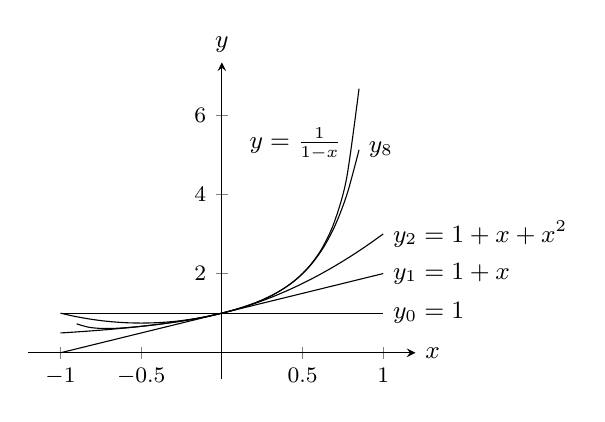
\begin{tikzpicture}[font=\small,declare function={fa(\x)=1;fb(\x)=1+\x;fc(\x)=1+\x+\x^2;fd(\x)=1+\x+\x^2+\x^3+\x^4+\x^5+\x^6+\x^7+\x^8;}]
\begin{axis}[clip=false,small,axis lines=middle, xlabel={$x$},ylabel={$y$},xlabel style={at={(current axis.right of origin)},anchor=west},ylabel style={at={(current axis.above origin)},anchor=south},enlargelimits=true]
\addplot[domain=-1:1]{fa(x)}node[right]{$y_0=1$};
\addplot[domain=-1:1]{fb(x)}node[right]{$y_1=1+x$};
\addplot[smooth,domain=-1:1]{fc(x)}node[right]{$y_2=1+x+x^2$};
\addplot[smooth,domain=-0.9:0.85]{fd(x)}node[right]{$y_8$};
\addplot[smooth,domain=-1:0.85]{1/(1-x)}node[pos=0.8,left]{$y=\frac{1}{1-x}$};
\end{axis}
\end{tikzpicture}
\caption{تفاعل \عددی{f(x)=\tfrac{1}{1-x}} اور اس کی چار تخمینی کثیر رکنیاں (مثال \حوالہ{مثال_تسلسل_تفاعل_اور_تخمینی_کثیر_رکنیاں_الف})۔}
\label{شکل_تسلسل_زیادہ_اجزاء_لینے_ہوں_گے}
\end{minipage}\hfill
\begin{minipage}{0.45\textwidth}
\centering
\begin{tikzpicture}[font=\small,declare function={f(\x)=1;fa(\x)=2-1/2*\x;fb(\x)=3-3/2*\x+1/4*\x^2;}]
\begin{axis}[clip=false,small,axis lines=middle, xlabel={$x$},ylabel={$y$},xlabel style={at={(current axis.right of origin)},anchor=west},ylabel style={at={(current axis.above origin)},anchor=south},enlargelimits=true,xmax=5]
\addplot[domain=0.25:3]{f(x)}node[pos=0.2,above]{$y_0=1$};
\addplot[domain=0.25:3.5]{fa(x)}node[pin=10:{$y_1=2-\frac{x}{2}$}]{};
\addplot[domain=0.75:3.5]{fb(x)}node[pin=80:{$y_1=3-\frac{3x}{2}+\frac{x^2}{4}$}]{};
\addplot[domain=0.75:3.5]{2/x}node[pin=30:{$y=\frac{2}{x}$}]{};
\draw(2,1)node[circ]{}node[below left]{$(2,1)$};
\end{axis}
\end{tikzpicture}
\caption{تفاعل \عددی{f(x)=\tfrac{2}{x}} اور اس کی ابتدائی تین تخمینی کثیر رکنیاں (مثال \حوالہ{مثال_تسلسل_تفاعل_اور_تخمینی_کثیر_رکنیاں_ب})۔}
\label{شکل_تسلسل_تفاعل_کی_تخمینی_کثیر_رکنیاں}
\end{minipage}
\end{figure}

\ابتدا{مثال}\شناخت{مثال_تسلسل_تفاعل_اور_تخمینی_کثیر_رکنیاں_ب}
درج ذیل طاقتی تسلسل مساوات \حوالہ{مساوات_تسلسل_تعریف_طاقتی_ب} کی طرح ہے جہاں \عددی{a=2}، \عددی{c_0=1}، \عددی{c_1=-\tfrac{1}{2}}، \عددی{c_2=\tfrac{1}{4}}، \نقطے،\عددی{c_n=(-1/2)^n} ہیں۔
\begin{align}\label{مساوات_تسلسل_تعریف_طاقتی_ت}
1-\frac{1}{2}(x-2)+\frac{1}{4}(x-2)^2+\cdots+\big(-\frac{1}{2}\big)^n(x-2)^n+\cdots
\end{align}
یہ ایک ہندسی تسلسل ہے جس کا ابتدائی جزو \عددی{1} اور نسبت \عددی{r=-\tfrac{x-2}{2}} ہے۔ یہ تسلسل \عددی{\abs{\tfrac{x-2}{2}}<1} یعنی \عددی{0<x<4} کے لئے مرکوز ہے۔اس کا مجموعہ
\begin{align*}
\frac{1}{1-r}=\frac{1}{1+\tfrac{x-2}{2}}=\frac{2}{x}
\end{align*}
ہے لہٰذا
\begin{align*}
\frac{2}{x}=1-\frac{1}{2}(x-2)+\frac{1}{4}(x-2)^2+\cdots+\big(-\frac{1}{2}\big)^n(x-2)^n+\cdots,\quad 0<x<4
\end{align*}
ہو گا۔ مساوات \حوالہ{مساوات_تسلسل_تعریف_طاقتی_ت} کا تسلسل \عددی{2} کے قریب \عددی{x} کی قیمتوں کے لئے  \عددی{f(x)=\tfrac{2}{x}} کی کارآمد تخمینی کثیر رکنیاں پیدا کرتا ہے (شکل \حوالہ{شکل_تسلسل_تفاعل_کی_تخمینی_کثیر_رکنیاں}):
\begin{align*}
P_0(x)&=1\\
P_1(x)&=1-\frac{1}{2}(x-2)=2-\frac{x}{2}\\
P_2(x)&=1-\frac{1}{2}(x-2)+\frac{1}{4}(x-2)^2=3-\frac{3x}{2}+\frac{x^2}{4}
\end{align*}
\انتہا{مثال}
%======================
\ابتدا{مثال}\شناخت{مثال_تسلسل_مرتکز_منفرج_تسلسل}
درج ذیل طاقتی تسلسل \عددی{x} کی کن قیمتوں کے لئے ارتکاز پذیر ہے؟
\begin{align*}
\sum_{n=1}^{\infty}(-1)^{n-1}\,\frac{x^n}{n}&=x-\frac{x^2}{2}+\frac{x^3}{3}-\cdots&&\text{\RL{(ا)}}\\
\sum_{n=1}^{\infty}(-1)^{n-1}\,\frac{x^{2n-1}}{2n-1}&=x-\frac{x^3}{3}+\frac{x^5}{5}-\cdots&&\text{\RL{(ب)}}\\
\sum_{n=0}^{\infty}\frac{x^n}{n!}&=1+x+\frac{x^2}{2!}+\frac{x^3}{3!}+\cdots&&\text{\RL{(ج)}}\\
\sum_{n=0}^{\infty}n!x^n&=1+x+2!x^2+3!x^3+\cdots&&\text{\RL{(د)}}
\end{align*}
حل:تناسبی پرکھ کا اطلاق تسلسل \عددی{\sum\abs{u_n}} پر کریں جہاں زیر غور تسلسل \عددی{n} جزو \عددی{u_n} ہے۔ نتائج شکل \حوالہ{شکل_مثال_تسلسل_مرتکز_منفرج_تسلسل} میں دکھائے گئے ہیں۔
\begin{enumerate}[a.]
\item
$\abs{\frac{u_{n+1}}{u_n}}=\frac{n}{n+1}\abs{x}\to\abs{x}$\\
 یہ تسلسل \عددی{\abs{x}<1} کے لئے مطلق مرتکز ہے۔ \عددی{\abs{x}>1} کے لئے چونکہ اس کا \عددی{n} واں جزو صفر تک نہیں پہنچتا لہٰذا تسلسل منفرج ہو گا جبکہ \عددی{x=1} پر ہمیں بدلتا ہارمونی تسلسل \عددی{1-\tfrac{1}{2}+\tfrac{1}{3}-\tfrac{1}{4}+\cdots} حاصل ہوتا ہے جو مرتکز ہے۔ \عددی{x=-1} پر ہمیں ہارمونی تسلسل کا نفی \عددی{-1-\tfrac{1}{2}-\tfrac{1}{3}-\tfrac{1}{4}-\cdots} ملتا ہے جو منفرج ہے۔ یوں تسلسل  (ا) وقفہ \عددی{-1<x\le 1} کے لئے مرتکز اور اس وقفہ کے باہر منفرج ہو گا۔
\item
$\abs{\frac{u_{n+1}}{u_n}}=\frac{2n-1}{2n+1}x^2\to x^2$\\
\عددی{x^2<1} کے لئے تسلسل مطلق مرتکز ہے۔ چونکہ \عددی{x^2>1} پر \عددی{n} واں جزو صفر پر مرکوز نہیں ہے لہٰذا تسلسل منفرج ہو گا۔ \عددی{x=1} پر تسلسل \عددی{1-\tfrac{1}{3}+\tfrac{1}{5}-\tfrac{1}{7}+\cdots} دیتا ہے جو مسئلہ بدلتا تسلسل کے تحت مرتکز ہو گا۔ \عددی{x=-1} پر بھی بدلتا تسلسل ملتا ہے جو ارتکاز کے شرائط کو مطمئن کرتا ہے لہٰذا یہ مرتکز ہو گا۔ نقطہ \عددی{x=1} پر تسلسل کی قیمت نقطہ \عددی{x=-1} پر تسلسل کی قیمت کا منفی ہے۔ تسلسل (ب) وقفہ \عددی{-1\le x\le 1} پر مرتکز جب کے اس کے باہر منفرج ہو گا۔
\item
$\abs{\frac{u_{n+1}}{u_n}}=\abs{\frac{x^{n+1}}{(n+1)!}\cdot\frac{n!}{x^n}}=\frac{\abs{x}}{n+1}\to 0$\\
تسلسل تمام \عددی{x} کے لئے مطلق مرتکز ہے۔
\item
$\abs{\frac{u_{n+1}}{u_n}}=\abs{\frac{(n+1)!x^{n+1}}{n!x^n}}=(n+1)\abs{x}\to\infty$\\
ماسوائے \عددی{x=0} تسلسل \عددی{x} کی تمام قیمتوں کے لئے منفرج ہو گا۔ 
\end{enumerate}
\انتہا{مثال}
%=====================
\begin{figure}
\centering
\begin{tikzpicture}
\draw(-1,0)--++(0,0.15)  (1,0)--++(0,0.15);
\draw[-latex](-1.5,0)node[left]{\RL{(ا)}}--(1.5,0)node[right]{$x$};
\draw[thick](-1,0)node[ocirc]{}node[below]{$-1$}--(1,0)node[circ]{}node[below]{$1$};
%
\draw(-1,-1)--++(0,0.15)  (1,-1)--++(0,0.15);
\draw[-latex](-1.5,-1)node[left]{\RL{(ب)}}--(1.5,-1)node[right]{$x$};
\draw[thick](-1,-1)node[circ]{}node[below]{$-1$}--(1,-1)node[circ]{}node[below]{$1$};
%
\begin{scope}[xshift=-6cm]
\draw[-latex](-1.5,0)node[left]{\RL{(ج)}}--(1.5,0)node[right]{$x$};
\draw[thick](-1.5,0)--(1.5,0);
\draw(0,0)node[below]{$0$}--++(0,0.15);
%
\draw[-latex](-1.5,-1)node[left]{\RL{(د)}}--(1.5,-1)node[right]{$x$};
\draw[](0,-1)node[circ]{}node[below]{$0$}--++(0,0.15);
\end{scope}
\end{tikzpicture}
\caption{وقفہ ارتکاز برائے مثال \حوالہ{مثال_تسلسل_مرتکز_منفرج_تسلسل}}
\label{شکل_مثال_تسلسل_مرتکز_منفرج_تسلسل}
\end{figure}
ہم نے مثال \حوالہ{مثال_تسلسل_مرتکز_منفرج_تسلسل} میں تسلسل کو ارتکاز یا انفراج کے لئے پرکھنا دیکھا۔ 


\ابتدا{پرکھ}\موٹا{طاقتی تسلسل کا پرکھ برائے ارتکاز}\\
قدم ا: تناسبی پرکھ (یا \عددی{n} واں جذر پرکھ) استعمال کرتے ہوئے وہ وقفہ تلاش کریں جس پر تسلسل مطلق مرتکز ہو۔ عموماً یہ وقفہ کھلا وقفہ ہو گا:
\begin{align*}
a-R<x<a+R\quad \text{یعنی}\quad\abs{x-a}<R
\end{align*}
قدم ب: اگر مطلق ارتکاز کا وقفہ متناہی ہو تب ہر آخری نقطہ پر ارتکاز یا انفراج کے لئے تسلسل کو پرکھیں (جیسا مثال \حوالہ{مثال_تسلسل_مرتکز_منفرج_تسلسل}-ا اور ب میں کیا گیا)۔ آپ تقابلی پرکھ، تکملی پرکھ یا بدلتا تسلسل پرکھ استعمال کر سکتے ہیں۔\\
قدم ج: اگر مطلق ارتکاز کا وقفہ \عددی{a-R<x<a+R} ہو تب \عددی{\abs{x-a}>R} کے لئے تسلسل منفرج ہو گا (تسلسل یہاں مشروط مرتکز بھی نہیں ہو گا) چونکہ \عددی{x} کی ان قیمتوں کے لئے \عددی{n} واں جزو صفر تک نہیں پہنچتا ہے۔
\انتہا{پرکھ}
%======================

\ابتدا{مسئلہ}\شناخت{مسئلہ_تسلسل_طاقتی_تسلسل_مسئلہ_ارتکاز}\موٹا{طاقتی تسلسل کا مسئلہ ارتکاز}\\
اگر \عددی{x=c\ne 0} کے لئے تسلسل \عددی{\sum_{n=0}^{\infty}a_nx^n=a_0+a_1x+a_2x^2+\cdots} مرتکز ہو تب \عددی{\abs{x}<\abs{c}} کے لئے یہ مطلق مرتکز ہو گا۔ اگر \عددی{x=d} کے لئے تسلسل منفرج ہو تب \عددی{\abs{x}>\abs{d}} کے لئے یہ منفرج ہو گا۔
\انتہا{مسئلہ}
%==========================

\ابتدا{ثبوت}
فرض کریں تسلسل \عددی{\sum_{n=0}^{\infty}a_nc^n} مرتکز ہے۔ تب \عددی{\lim_{n\to\infty}a_nc^n=0} ہو گا۔ یوں ایسا عدد \عددی{N} پایا جائے گا کہ تمام \عددی{n\ge N} کے لئے \عددی{\abs{a_nc^n}<1} ہو گا، یعنی:
\begin{align}\label{مساوات_مسئلہ_ارتکاز_ثبوت_الف}
\abs{a_n}&<\frac{1}{\abs{c^n}}&& n\ge N
\end{align}
اب ایسا \عددی{x} لیں کہ \عددی{\abs{x}<\abs{c}} ہو اور درج ذیل پر غور کریں۔
\begin{align*}
\abs{a_0}+\abs{a_1x}+\abs{a_{N-1}\,x^{N-1}}+\abs{a_N\,x^N}+\abs{a_{N+1}\,x^{N+1}}+\cdots
\end{align*}
جزو \عددی{\abs{a_N\,x^N}} سے قبل متناہی تعداد کے اجزاء پائے جاتے ہیں اور ان کا مجموعہ متناہی ہے۔ مساوات \حوالہ{مساوات_مسئلہ_ارتکاز_ثبوت_الف} کی بنا  جزو \عددی{\abs{a_N\,x^N}} اور اس کے بعد تمام اجزاء درج ذیل سے کم ہوں گے۔
\begin{align}\label{مساوات_مسئلہ_ارتکاز_ثبوت_ب}
\abs{\frac{x}{c}}^N+\abs{\frac{x}{c}}^{N+1}+\abs{\frac{x}{c}}^{N+2}+\cdots
\end{align}
اب مساوات \حوالہ{مساوات_مسئلہ_ارتکاز_ثبوت_ب} ہندسی تسلسل ہے  جس کا نسبت \عددی{r=\abs{\tfrac{x}{c}}} ہے جو \عددی{\abs{x}<\abs{c}} کی بنا \عددی{1} سے کم ہے۔ یوں مساوات \حوالہ{مساوات_مسئلہ_ارتکاز_ثبوت_ب} کا تسلسل مرتکز ہے لہٰذا اصل تسلسل مطلق مرتکز ہو گا۔ یوں مسئلے کا پہلا حصہ ثابت ہوتا ہے۔

مسئلے کا دوسرا حصہ مسئلے کے پہلے حصہ سے حاصل ہوتا ہے۔ اگر \عددی{x=d} کے لئے تسلسل منفرج اور \عددی{x_0} پر تسلسل مرتکز ہو جہاں \عددی{\abs{x_0}>\abs{d}} ہے تب ہم مسئلے کے پہلے حصے میں \عددی{c=x_0} لے کر فیصلہ کر سکتے ہیں کہ \عددی{d} پر تسلسل مطلق مرتکز ہو گا، لیکن ایک ہی وقت میں تسلسل مرتکز اور منفرج دونوں  نہیں ہو سکتا ہے۔ یوں اگر تسلسل \عددی{d} پر منفرج ہو تب تمام \عددی{\abs{x}>\abs{d}} کے لئے یہ  منفرج ہو گا۔
\انتہا{ثبوت}
%=====================

علامتیت  سادہ رکھنے کی خاطر مسئلہ \حوالہ{مسئلہ_تسلسل_طاقتی_تسلسل_مسئلہ_ارتکاز} میں تسلسل \عددی{\sum a_nx^n}  کے ارتکاز کی بات کی گئی۔ تسلسل \عددی{\sum a_n(x-a)^n} کے ارتکاز کی بات کرتے ہوئے ہم \عددی{x-a} کی جگہ \عددی{x'} پر کر کے نتیجہ کو تسلسل \عددی{\sum a_n(x')^n} پر لاگو کر سکتے ہیں۔

\جزوحصہء{ارتکاز کا رداس اور وقفہ}
اب تک دیکھے گئے مثالوں اور مذکورہ بالا مسئلے کو دیکھ کر ہم کہہ سکتے ہیں کہ طاقتی تسلسل کا رویہ درج ذیل میں سے ایک ہو گا۔

\موٹا{تسلسل \عددی{\sum c_n(x-a)^n} کے ممکنہ رویے}
\begin{enumerate}[a.]
\item
ایک ایسا مثبت عدد \عددی{R} پایا جاتا ہے کہ \عددی{\abs{x-a}>R} کے لئے تسلسل منفرج جبکہ \عددی{\abs{x-a}<R} کے لئے مطلق مرتکز ہے۔ ہر ایک آخری نقطہ \عددی{x=a-R} اور \عددی{x=a+R} پر تسلسل مرتکز یا منفرج ہو سکتا ہے۔ 
\item
ہر \عددی{x} پر تسلسل مطلق مرتکز ہے (\عددی{R=\infty})۔
\item
تسلسل \عددی{x=a} کے لئے مرتکز جبکہ باقی تمام \عددی{x} کے لئے منفرج ہے (\عددی{R=0})۔
\end{enumerate}

پہلی صورت میں ارتکاز کے نقطوں کا سلسلہ متناہی وقفہ ہے جس کو \اصطلاح{وقفہ ارتکاز}\فرہنگ{ارتکاز!وقفہ}\حاشیہب{interval of convergence}\فرہنگ{convergence!interval} کہتے ہیں۔ ہم مذکورہ بالا مثالوں سے جانتے ہیں کہ وقفہ ارتکاز کھلا، نصف کھلا، یا بند ہو سکتا ہے اور یہ دیے گئے تسلسل پر منحصر ہو گا۔ وقفہ ارتکاز جس قسم کا بھی ہو، \عددی{R} کو تسلسل کا \اصطلاح{رداس ارتکاز}\فرہنگ{ارتکاز!رداس}\حاشیہب{radius of convergence}\فرہنگ{convergence!radius} کہیں گے اور تسلسل کے ان نقطوں کا سلسلہ، جن کے لئے تسلسل مرتکز ہو، کا کم سے کم بالائی حد بندی  \عددی{a+R} ہو گا۔ اس وقفہ کی اندرونی ہر نقطہ پر ارتکاز مطلق ہو گا۔اگر \عددی{x} کی تمام مثبت قیمتوں کے لئے ایک تسلسل مطلق مرتکز ہو تب ہم کہتے ہیں اس تسلسل کا \اصطلاح{رداس ارتکاز لامتناہی}\فرہنگ{رداس ارتکاز!لامتناہی} ہے۔ اگر یہ صرف \عددی{x=a} کے لئے مرتکز ہو تب اس کا \اصطلاح{رداس ارتکاز صفر}\فرہنگ{رداس ارتکاز!صفر} ہو گا۔ 

\جزوحصہء{جزو در جزو تفرق}
اعلٰی احصاء کا یک مسئلہ کہتا ہے کہ وقفہ ارتکاز کے اندر ہر نقطہ پر طاقتی تسلسل کا جزو در جزو تفرق لیا جا سکتا ہے۔

\ابتدا{مسئلہ}\شناخت{مسئلہ_تسلسل_جزو_در_جزو_طاقتی_تفرق}\موٹا{مسئلہ جزو در جزو تفرق}\\
وقفہ  \عددی{a-R<x<a+R} پر مرتکز تسلسل \عددی{\sum c_n(x-a)^n} درج ذیل تفاعل \عددی{f} دیتا کرتا ہے، جہاں \عددی{R>0} ہے۔
\begin{align*}
f(x)&=\sum_{n=0}^{\infty}c_n(x-a)^n&&a-R<x<a+R
\end{align*}
وقفہ ارتکاز کے اندر ایسے تفاعل کا ہر رتبے کا تفرق پایا جاتا ہے۔ ان تفرق کو حاصل کرنے کے لئے ہم اصل تسلسل کا جزو در جزو تفرق
\begin{align*}
f'(x)&=\sum_{n=1}^{\infty}nc_n(x-a)^{n-1}\\
f''(x)&=\sum_{n=2}^{\infty}n(n-1)c_nx^{n-2}
\end{align*}
لیتے ہیں، وغیرہ وغیرہ۔اصل تسلسل کے وقفہ ارتکاز کے ہر اندرونی نقطہ کے لئے یہ تفرقی تسلسل مرتکز ہوں گے۔
\انتہا{مسئلہ}
%============================ 

انتباہ: ضروری نہیں کہ جزو در جزو تفرق دیگر تسلسل کے لئے بھی قابل استعمال ہو۔ مثال کے طور پر تکونیاتی تسلسل \عددی{\sum_{n=1}^{\infty}\tfrac{\sin(n!x)}{n^2}} تمام \عددی{x} کے لئے مرتکز ہے۔ البتہ اس کا جزو در جزو تفرق \عددی{\sum_{n=1}^{\infty}\tfrac{n!\cos(n!x)}{n^2}}  ہے جو تمام \عددی{x} کے لئے منفرج ہے۔

\ابتدا{مثال}
درج ذیل تفاعل \عددی{f(x)} کے تفرق \عددی{f'(x)} اور \عددی{f''(x)} حاصل کریں۔
\begin{align*}
f(x)&=\frac{1}{1-x}=1+x+x^2+x^3+x^4+\cdots+x^n+\cdots\\
&=\sum_{n=0}^{\infty}x^n&&-1<x<1
\end{align*}
حل:\quad
\begin{align*}
f'(x)=\frac{1}{(1-x)^2}&=1+2x+3x^2+4x^3+\cdots+nx^{n-1}+\cdots\\
&=\sum_{n=1}^{\infty}nx^{n-1}&&-1<x<1\\
f''(x)=\frac{2}{(1-x)^3}&=2+6x+12x^2+\cdots+n(n-1)x^{n-2}+\cdots\\
&=\sum_{n=2}^{\infty}n(n-1)x^{n-2}&&-1<x<1
\end{align*}
\انتہا{مثال}
%==========================

\جزوحصہء{جزو در جزو تکمل}
اعلٰی احصاء کا دوسرا مسئلہ کہتا ہے کہ پورے وقفہ ارتکاز کے اندر  طاقتی تسلسل کا جزو در جزو تکمل لیا جا سکتا ہے۔

\ابتدا{مسئلہ}\موٹا{مسئلہ جزو در جزو تکمل}\\
فرض کریں \عددی{a-R<x<a+R\,\, (R>0)} میں 
\begin{align*}
f(x)=\sum_{n=0}^{\infty}c_n(x-a)^n
\end{align*}
مرتکز ہو تب \عددی{a-R<x<a+R} میں 
\begin{align*}
\sum_{n=0}^{\infty}\frac{c_n(x-a)^{n+1}}{n+1}
\end{align*}
مرتکز ہو گا  اور \عددی{a-R<x<a+R} میں درج ذیل ہو گا۔
\begin{align*}
\int f(x)\dif x=\sum_{n=0}^{\infty}c_n\frac{(x-a)^{n+1}}{n+1}+C
\end{align*}
\انتہا{مسئلہ}
%===================

\ابتدا{مثال}\شناخت{مثال_تسلسل_الٹ_ٹینجنٹ_کا_تسلسل}\ترچھا{وقفہ \عددی{-1\le x\le 1} میں \عددی{\tan^{-1}x} کا تسلسل}\\
درج ذیل تفاعل پہچانیں۔
\begin{align*}
f(x)&=x-\frac{x^3}{3}+\frac{x^5}{5}-\cdots&&-1\le x\le 1
\end{align*}
حل:\quad
ہم اصل تسلسل کا جزو در جزو تفرق لیتے ہیں۔
\begin{align*}
f'(x)&=1-x^2+x^4-x^6+\cdots&&-1\le x\le 1
\end{align*}
یہ ہندسی تسلسل ہے جس کا پہلا جزو \عددی{1} اور نسبت \عددی{-x^2} ہے لہٰذا
\begin{align*}
f'(x)=\frac{1}{1-(-x^2)}=\frac{1}{1+x^2}
\end{align*}
ہو گا۔ہم اب \عددی{f'(x)=\tfrac{1}{1+x^2}} کا تکمل لیتے ہیں۔
\begin{align*}
\int f'(x)\dif x=\int\frac{\dif x}{1+x^2}=\tan^{-1}x+C
\end{align*}
چونکہ \عددی{x=0} پر \عددی{f(x)} کا تسلسل صفر ہے لہٰذا \عددی{C=0} ہو گا۔یوں درج ذیل ہو گا۔
\begin{align}
f(x)&=x-\frac{x^3}{3}+\frac{x^5}{5}-\frac{x^7}{7}+\cdots=\tan^{-1}x&&-1<x<1
\end{align}
\انتہا{مثال}
%==================

ہم دیکھیں گے کہ \عددی{x=\mp 1} کے لئے بھی یہ تسلسل \عددی{\tan^{-1}x} پر مرکوز ہے۔

ہم دیکھتے ہیں کہ مثال \حوالہ{مثال_تسلسل_الٹ_ٹینجنٹ_کا_تسلسل} میں اصل تسلسل کے وقفہ ارتکاز کے   دونوں آخری نقطوں کے لئے اصل تسلسل مرتکز ہے، البتہ مسئلہ \حوالہ{مسئلہ_تسلسل_جزو_در_جزو_طاقتی_تفرق} صرف اصل تسلسل کے وقفہ ارتکاز کی اندرون میں تفرقی تسلسل کے ارتکاز کی ضمانت دیتا ہے۔

\ابتدا{مثال}\موٹا{وقفہ \عددی{-1<x<1} کے لئے \عددی{\ln (1+x)} کا تسلسل}\\
کھلا وقفہ \عددی{-1<t<1} کے لئے تسلسل
\begin{align*}
\frac{1}{1+t}=1-t+t^2-t^3+\cdots
\end{align*}
 مرکوز ہے۔یوں درج ذیل ہو گا۔
\begin{align*}
\ln(1+x)&=\int_0^x\frac{1}{1+t}\dif t=\left. t-\frac{t^2}{2}+\frac{t^3}{3}-\frac{t^4}{4}+\cdots\right]_0^x\\
&=x-\frac{x^2}{2}+\frac{x^3}{3}-\frac{x^4}{4}+\cdots&&-1<x<1
\end{align*}
\انتہا{مثال}
%=======================
یہ دکھایا جا سکتا ہے کہ \عددی{x=1} پر تسلسل عدد \عددی{\ln2} کو مرکوز ہے  مگر مسئلہ اس کی ضمانت نہیں دیتا ہے۔

\جزوحصہء{فنیات}

